\documentclass{article}

\usepackage{graphicx}
\usepackage{tikz}
\usepackage{tikzsymbols}
\usetikzlibrary{calc,patterns,shapes.geometric}
\pagestyle{empty}
\usepackage[margin=0pt]{geometry}
\geometry{papersize={14in,12in}}

\def\centerarc[#1](#2)(#3:#4:#5){\draw[#1] ($(#2)+({#5*cos(#3)},{#5*sin(#3)})$) arc (#3:#4:#5);}

\begin{document}
	\begin{figure}
		\centering
		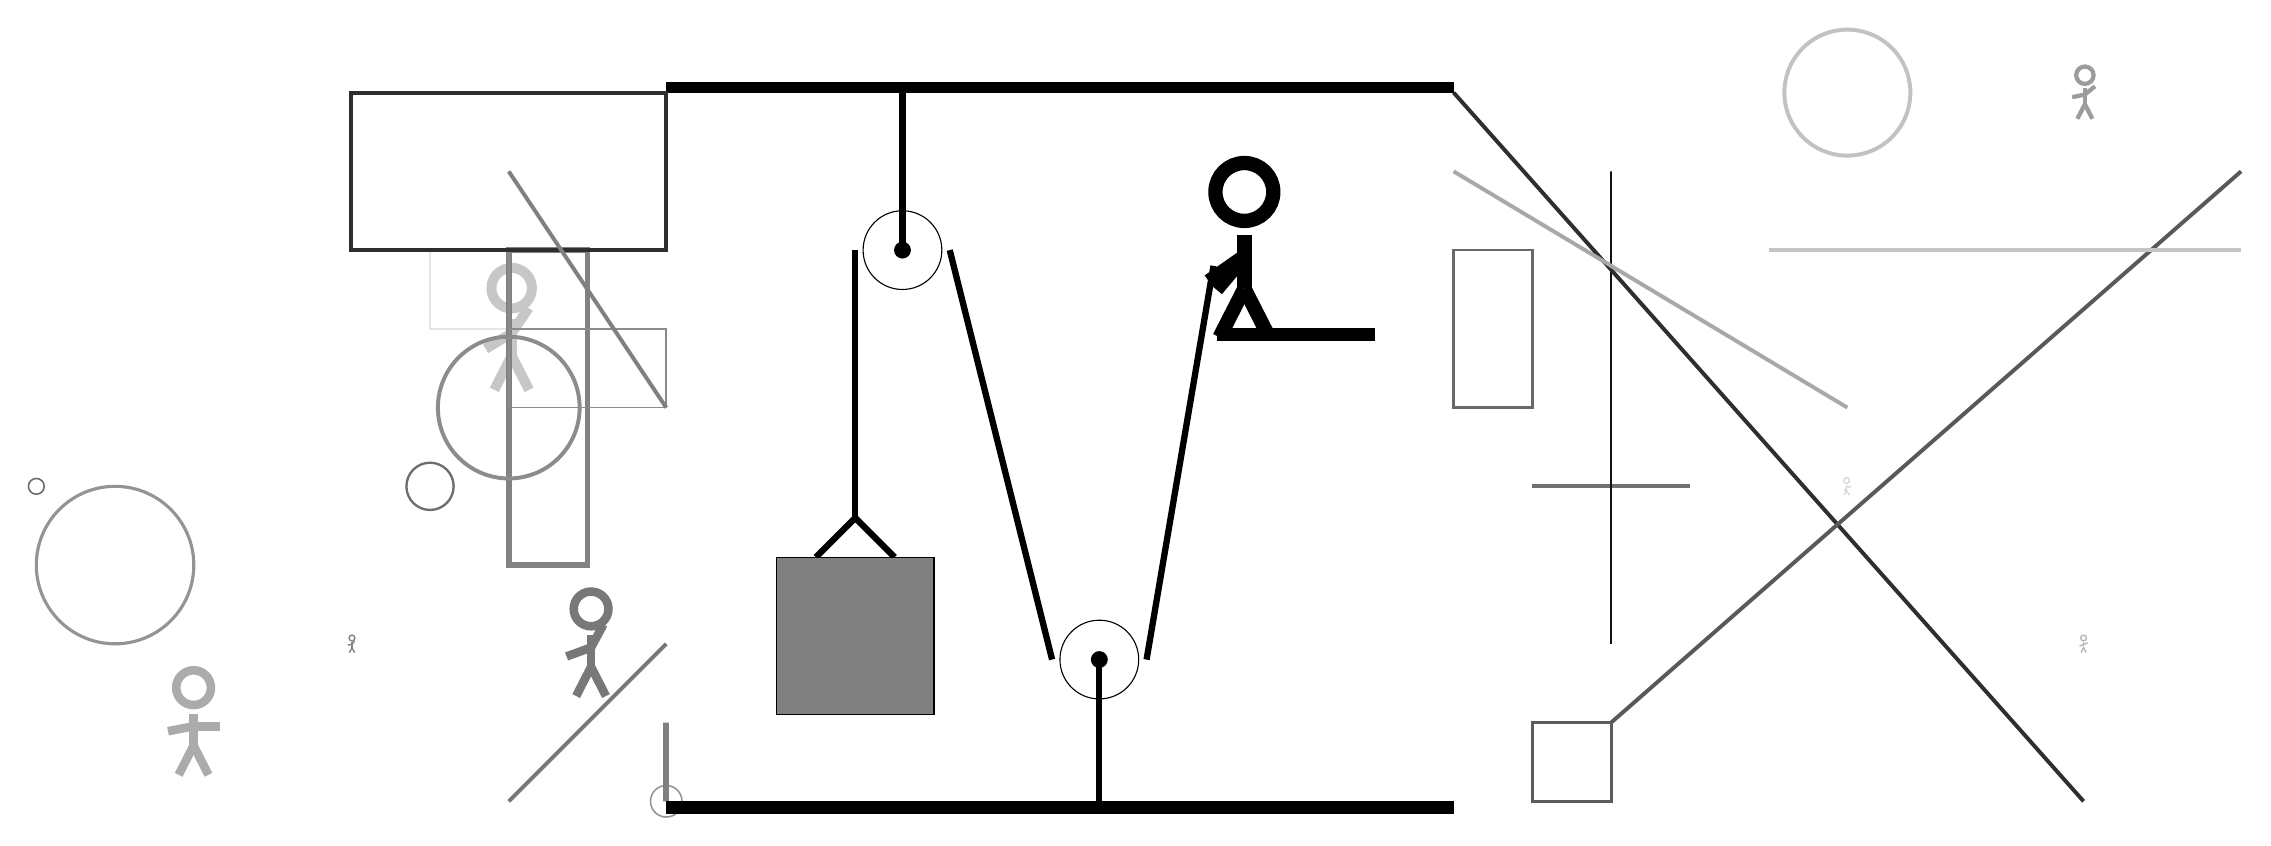
\begin{tikzpicture}
			%%%%% START %%%%%
			
			\draw[fill=black] (-2, 9) rectangle (8, 9.125);
			
			\draw (3.5, 1.8) circle (0.5);
			\draw[fill=black] (3.5, 1.8) circle (0.1);
			\draw[line width=0.8mm] (3.5, 1.8) -- (3.5, 0);
			
			\draw (1, 7) circle (0.5);
			\draw[fill=black] (1, 7) circle (0.1);
			\draw[line width=0.8mm] (1, 9) -- (1, 7);
			
			\draw[line width=0.8mm](-0.1, 3.1) --  (0.4, 3.6) -- (0.9, 3.1);
			\draw[fill=black!50] (-0.6, 3.1) rectangle (1.4, 1.1);
			
			\node[line width=0.4mm, color=black!22] at (-4, 6) {\Strichmaxerl[7][31][56]};
			
			\node[line width=0.7mm, color=black!15] at (13, 4) {\Strichmaxerl[1][66][1]};
			\draw[line width=0.3mm, color=black!10] (-4, 6) rectangle (-5, 7);
			\draw[line width=0.7mm, color=black!49] (-3, 7) rectangle (-4, 3);
			
			\draw [line width=0.4mm, color=black!42](-9, 3) circle (1.0);
			\node[line width=0.4mm, color=black!39] at (16, 9) {\Strichmaxerl[3][12][39]};
			\draw[line width=0.2mm, color=black!45] (-4, 6) rectangle (-2, 5);
			\draw [line width=0.2mm, color=black!42](-2, 0) circle (0.2);
			\draw [line width=0.5mm, color=black!24](13, 9) circle (0.8);
			\draw [line width=0.3mm, color=black!57](-5, 4) circle (0.3);
			
			\draw [line width=0.2mm, color=black!58](-10, 4) circle (0.1);
			
			\draw[line width=0.3mm, color=black!45] (-4, 5) rectangle (-4, 7);
			\draw[line width=0.5mm, color=black!53](-2, 2) -- (-4, 0);
			\draw [line width=0.4mm, color=black!20](10, 2) circle (0.0);
			\draw[line width=0.5mm, color=black!82] (-2, 9) rectangle (-6, 7);
			\draw[line width=0.5mm, color=black!56](9, 4) -- (11, 4);
			
			\draw[line width=0.2mm, color=black!93] (10, 2) rectangle (10, 8);
			\draw [line width=0.5mm, color=black!45](-4, 5) circle (0.9);
			\node[line width=0.4mm, color=black!53] at (-3, 2) {\Strichmaxerl[6][20][62]};
			\node[line width=0.6mm, color=black!49] at (-6, 2) {\Strichmaxerl[1][8][54]};
			\draw[line width=0.5mm, color=black!82](8, 9) -- (16, 0);
			
			\node[line width=0.7mm, color=black!33] at (-8, 1) {\Strichmaxerl[6][11][0]};
			\draw[line width=0.5mm, color=black!50](-2, 5) -- (-4, 8);
			\draw[line width=0.3mm, color=black!59] (9, 5) rectangle (8, 7);
			\draw[line width=0.5mm, color=black!65](10, 1) -- (18, 8);
			\draw[line width=0.5mm, color=black!34](13, 5) -- (8, 8);
			\draw[line width=0.4mm, color=black!64] (9, 1) rectangle (10, 0);
			\node[line width=0.7mm, color=black!28] at (16, 2) {\Strichmaxerl[1][22][21]};
			\draw[line width=0.7mm, color=black!50] (-2, 1) rectangle (-2, 0);
			\draw[line width=0.5mm, color=black!23](12, 7) -- (18, 7);
			
			\draw[line width=0.8mm](0.4, 7) -- (0.4, 3.6);
			\centerarc[line width=0.8mm](1, 7)(180:0:0.6)
			\draw[line width=0.8mm](1.6, 7) -- (2.9, 1.8);
			\centerarc[line width=0.8mm](3.5, 1.8)(180:360:0.6)
			\draw[line width=0.8mm](4.1, 1.8) -- (4.95, 6.8);
			
			\node at (5.3, 7) {\Strichmaxerl[10][35][-130]};
			\draw[fill=black] (5, 6) rectangle (7, 5.85);
			
			\draw[fill=black] (-2, 0) rectangle (8, -0.15);
			
			%%%%% END %%%%%
		\end{tikzpicture}
	\end{figure}	
\end{document}